%% This file was auto-generated by IPython.
%% Conversion from the original notebook file:
%% stat_AtA_qr.ipynb
%%
\documentclass[11pt,english,fleqn]{article}

%% This is the automatic preamble used by IPython.  Note that it does *not*
%% include a documentclass declaration, that is added at runtime to the overall
%% document.

\usepackage{amsmath}
\usepackage{amssymb}
\usepackage{graphicx}
\usepackage{ucs}
\usepackage[utf8x]{inputenc}

% needed for markdown enumerations to work
\usepackage{enumerate}

% Slightly bigger margins than the latex defaults
\usepackage{geometry}
\geometry{verbose,tmargin=3cm,bmargin=3cm,lmargin=2.5cm,rmargin=2.5cm}

% Define a few colors for use in code, links and cell shading
\usepackage{color}
\definecolor{orange}{cmyk}{0,0.4,0.8,0.2}
\definecolor{darkorange}{rgb}{.71,0.21,0.01}
\definecolor{darkgreen}{rgb}{.12,.54,.11}
\definecolor{myteal}{rgb}{.26, .44, .56}
\definecolor{gray}{gray}{0.45}
\definecolor{lightgray}{gray}{.95}
\definecolor{mediumgray}{gray}{.8}
\definecolor{inputbackground}{rgb}{.95, .95, .85}
\definecolor{outputbackground}{rgb}{.95, .95, .95}
\definecolor{traceback}{rgb}{1, .95, .95}

% Framed environments for code cells (inputs, outputs, errors, ...).  The
% various uses of \unskip (or not) at the end were fine-tuned by hand, so don't
% randomly change them unless you're sure of the effect it will have.
\usepackage{framed}

% remove extraneous vertical space in boxes
\setlength\fboxsep{0pt}

% codecell is the whole input+output set of blocks that a Code cell can
% generate.

% TODO: unfortunately, it seems that using a framed codecell environment breaks
% the ability of the frames inside of it to be broken across pages.  This
% causes at least the problem of having lots of empty space at the bottom of
% pages as new frames are moved to the next page, and if a single frame is too
% long to fit on a page, will completely stop latex from compiling the
% document.  So unless we figure out a solution to this, we'll have to instead
% leave the codecell env. as empty.  I'm keeping the original codecell
% definition here (a thin vertical bar) for reference, in case we find a
% solution to the page break issue.

%% \newenvironment{codecell}{%
%%     \def\FrameCommand{\color{mediumgray} \vrule width 1pt \hspace{5pt}}%
%%    \MakeFramed{\vspace{-0.5em}}}
%%  {\unskip\endMakeFramed}

% For now, make this a no-op...
\newenvironment{codecell}{}

 \newenvironment{codeinput}{%
   \def\FrameCommand{\colorbox{inputbackground}}%
   \MakeFramed{\advance\hsize-\width \FrameRestore}}
 {\unskip\endMakeFramed}

\newenvironment{codeoutput}{%
   \def\FrameCommand{\colorbox{outputbackground}}%
   \vspace{-1.4em}
   \MakeFramed{\advance\hsize-\width \FrameRestore}}
 {\unskip\medskip\endMakeFramed}

\newenvironment{traceback}{%
   \def\FrameCommand{\colorbox{traceback}}%
   \MakeFramed{\advance\hsize-\width \FrameRestore}}
 {\endMakeFramed}

% Use and configure listings package for nicely formatted code
\usepackage{listingsutf8}
\lstset{
  language=python,
  inputencoding=utf8x,
  extendedchars=\true,
  aboveskip=\smallskipamount,
  belowskip=\smallskipamount,
  xleftmargin=2mm,
  breaklines=true,
  basicstyle=\small \ttfamily,
  showstringspaces=false,
  keywordstyle=\color{blue}\bfseries,
  commentstyle=\color{myteal},
  stringstyle=\color{darkgreen},
  identifierstyle=\color{darkorange},
  columns=fullflexible,  % tighter character kerning, like verb
}

% The hyperref package gives us a pdf with properly built
% internal navigation ('pdf bookmarks' for the table of contents,
% internal cross-reference links, web links for URLs, etc.)
\usepackage{hyperref}
\hypersetup{
  breaklinks=true,  % so long urls are correctly broken across lines
  colorlinks=true,
  urlcolor=blue,
  linkcolor=darkorange,
  citecolor=darkgreen,
  }

% hardcode size of all verbatim environments to be a bit smaller
\makeatletter 
\g@addto@macro\@verbatim\small\topsep=0.5em\partopsep=0pt
\makeatother 

% Prevent overflowing lines due to urls and other hard-to-break entities.
\sloppy

\setlength{\mathindent}{0pt}
\setlength{\parindent}{0pt}
\setlength{\parskip}{8pt}
\begin{document}

\section{Paralel Matris Çarpımı, Ax, QR ve SVD}

Matris Çarpımı adli yazi tek makinali ortamda matris carpiminin nasil
yapilacagini, ve nasil gorulecebilegini anlatti. Satir bakis acisi,
kolon bakis acisi islendi. Parallel (Hadoop), esle/indirge ortaminda
matris carpimini nasil yapariz? Mesela $A^TA$'yi ele alalim. Bu carpim
oldukca onemli cunku baska sonuclar icin de kullanilabiliyor. Mesela $A$
uzerinde $QR$ ayristirmasi yapmak isterseniz (bkz. Lineer Cebir ders
notlarimiz) bu carpim kullanilabiliyor.

Nasil? QR ayristirmasi kolonlarin hepsi bilindigi gibi birbirine dik
(orthogonal) birim vektorler olan bir $Q$ matrisi ve ust ucgensel (upper
triangular) bir $R$ matrisi olusturur. Ayristirmanin $A^TA$ ile
baglantisi nedir? Eger $A$ yerine onun ayristirmasini $QR$ koyarsak,
\[
A^TA = (QR)^T (QR) = R^T Q^T QR
\]
Tum $Q$ vektorleri birbirine dik, ve birim vektorler ise, $Q^T Q$ birim
matrisi $I$ olur. O zaman
\[
R^T Q^T QR = R^T R
\]
Yani
\[
A^TA = R^TR
\]
Bu muthis bir sonuc. Demek ki $A^TA$ carpimini yaptigimiz anda, bir
yandan $R^TR$ carpim sonucunu da hesaplamis oluyoruz.

Peki $A^TA$ hesaplayip (boylece $R^TR$'yi elde edince) onun icinden
$R$'yi nasil cekip cikartiriz?

Simdi Cholesky ayristirmasi kullanmanin zamani. Cholesky ayristirmasi
(herhangi bir $A$ matrisi uzerinde)
\[A = LL^T\]
olarak bilinir, yani bir matris alt ucgensel (lower triangular -ki L
harfi oradan geliyor-) $L$ matrisine ve onun devrigi olan ust ucgensel
$L^T$'nin carpimina ayristirilir. Elimizde $R^TR$ var, ve ona benzer
$LL^T$ var, $R$ bilindigi gibi ust ucgensel, $L$ alt ucgensel, $L^T$ ve
$R$ birbirine esit demek ki.

Yani $A^TA$ uzerinde numerik hesap kutuphenimzin Cholesky cagrisi
kullanmak bize $QR$'in $R$'sini verir.

Su anda akla su soru gelebilir: madem kutuphane cagrisi yaptik, niye $A$
uzerinde kutuphenimizin $QR$ cagrisini kullanmiyoruz?

Cevap Buyuk Veri argumaninda sakli. Bu ortamda ugrasilan verilerde $A$
matrisi $m \times n$ boyutlarindadir, ve $m$ milyonlar, hatta
milyarlarca satir olabilir. Simdilik $m >> n$ oldugunu farzedelim, yani
$m$, $n$'den ``cok, cok buyuk'', yani ``boyut kolonlarinin'', ki $n$,
sayisi binler ya da onbinlerde. Bu gayet tipik bir senaryo aslinda,
olcum noktalari (boyutlar) var, ama cok fazla degil, diger yandan o
olcumler icin milyonlarca veri noktasi toplanmis. Tipik bir asiri
belirtilmis (overdetermined) sistem - ki en az kareler (least squares)
gibi yaklasimlarin temel aldigi sistemler bunlardir, eldeki denklem
sayisindan daha fazla olcum noktasi vardir. Bu arada en az karelerden
bahsettik, $QR$'in kullanildigi alanlardan biri en az karelerin
cozumudur.

Argumana devam ediyoruz, kutuphane qr cagrisini $A$ uzerinde yaparsak,
$m \times n$ gibi devasa bir matris uzerinde islem yapmak gerekir. Ama
$A^TA$ uzerinde islem (Cholesky) yaparsak, ki bu carpimin boyutu
$n \times m \cdot m \times n = n \times n$, yani cok daha ufak bir
matristir. $A^TA$'in islem bedeli cok ufak, birazdan anlatacagimiz
yontem sayesinde bu bedel $O(m)$.

\subsubsection{Paralel $A^TA$}

Paralel carpima gelelim. Oncelikle elimizdeki becerilere (capabilities)
bakalim. Hadoop ortami bize asiri buyuk bir dosyayi otomatik olarak
makinalara bolerek bir hesap yapilmasi gerektiginde o hesabin her
makinada, elindeki veri parcasi uzerinde yaptirilmasini sagliyor.

$A^TA$ orneginde eldeki veri $A$, ve ``cok olan'' $A$'nin satirlari,
yani $m \times n$ boyutlarinda matris var ve $m$ devasa boyutlarda
(olabilir). Bir $A$ dosyasi tipik olarak soyle gozukecek:

\begin{codecell}
\begin{codeinput}
\begin{lstlisting}
!head -5 A_matrix
\end{lstlisting}
\end{codeinput}
\begin{codeoutput}
\begin{verbatim}
3 4 5 6
3 4 5 2
3 6 7 8
2 2 2 2
9 9 3 3
\end{verbatim}
\end{codeoutput}
\end{codecell}
Esle/indirgeye gelelim: Eger carpima satir bakisini hatirlarsak,

\begin{codecell}
\begin{codeinput}
\begin{lstlisting}
im=imread("AtA.png"); imshow(im)
\end{lstlisting}
\end{codeinput}
\begin{codeoutput}
\begin{verbatim}
<matplotlib.image.AxesImage at 0x3813890>
\end{verbatim}
\begin{center}
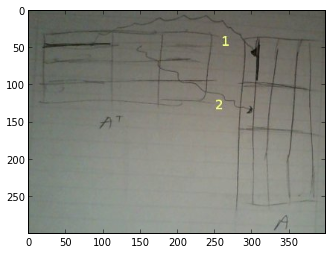
\includegraphics[width=0.7\textwidth]{stat_AtA_qr_files/stat_AtA_qr_fig_00.png}
\par
\end{center}
\end{codeoutput}
\end{codecell}
Bu bakisa gore soldaki matriste satir boyunca giderken, sagdakinde ona
tekabul eden kolon boyunca gidiyoruz, ve birbirine eslene her ogeyi
carpiyoruz, ve carpimlari topluyoruz.

Simdi bu matrisin Hadoop'ta parca parca bize geldigini dusunursek (ki
ustte hayali bir ilk parcayi kirmizi cizgi ile belirttik), bu parca
icinde mesela ilk satiri kendisi ile carparken (1'inci ok) ayni blok
icindeyiz. Bu onemli bir nokta, carparken bloklar arasi gecis yok.

Tabii ki nihai carpimdaki (1,1) hesabi icin $A^T$'deki birinci satirin
tamamen $A$'daki birinci kolonla nokta carpiminin bitirilmis olmasi
gerekir, ama simdi dusunelim, baska bir makinaya ikinci parca verilmis
ise, makinada o birinci satirin geri kalani carpilip toplanacaktir (2.
ok), ve eger tum parcalar, tum makinalarda bu sekilde islenirse, (1,1)
hesabi icin o makinalardaki o tum carpimlari alip nihai bir noktada
toplamak bize (1,1) icin nihai sonucu verecektir. Bu tipik bir
esle/indirge hesabi olabilir, esle safhasinda eldeki parca $A_p$
uzerinde $A_p^T A_p$ yapilir, indirge safhasinda bu parcalar toplanir.

Esleme safhasindan yayinlanacak (emit) anahtar ve degerler, bizce,
$A_p^T A_p$ icindeki her satirin satir no'su ve satir degeri olmali.
Niye? (Ayni sabit bir anahtar degeriyle beraber $A_p^T A_p$'in tamamini
da yayinlayabilirdik).

Hatirlayalim, nihai carpim $n \times n$ boyutunda, her parca $p$ olsa
bile, $n \times p \cdot p \times n$ yine bize $n \times n$ veriyor. Yani
her makina $n \times n$ boyutunda bir carpim sonucunu uretiyor. Evet $n$
nispeten kucuk bir sayi, fakat yine de onbinlerde olsa bile
$10,000 \times 10,000$ mesela, buyuk bir sayi. Eger tum toplami tek bir
indirgeyici makinaya yaptirirsak, pek cok $n \times n$ boyutunda
matrisin toplami bu makinayi kasar. O sebeple indirgeme sonrasi
matrisleri degil, o matrislerin her $n$ satirini satir no'su ile
yayinliyoruz, boylece ayni satirlar ayni indirgeyiciye gidip orada
toplaniyorlar, ama bircok indirgeyici var yani toplama islemi paralel
hale gelmis oluyor. Tabii indirgeme sonrasi o sonuclar yayinlaniyor, ve
satir no'ya gore dogal olarak siralanmis halde nihai sonuc cikiyor. Ama
toplama islemi paralel. Kod alttaki gibi

\begin{codecell}
\begin{codeinput}
\begin{lstlisting}
print(open("AtA.py").read())
\end{lstlisting}
\end{codeinput}
\begin{codeoutput}
\begin{verbatim}
from mrjob.job import MRJob
from mrjob.protocol import PickleProtocol
import numpy as np, sys

class MRAtA(MRJob):
    INTERNAL_PROTOCOL = PickleProtocol
    
    def __init__(self, *args, **kwargs):
        super(MRAtA, self).__init__(*args, **kwargs)
        self.buffer_size = 4
        self.n = 4
        self.data = []
        self.A_sum = np.zeros((self.n,self.n))
        
    def mapper(self, key, line):
        line_vals = map(np.float,line.split())
        self.data.append(line_vals)
        if len(self.data) == self.buffer_size:
            mult = np.dot(np.array(self.data).T,np.array(self.data))
            self.data = []
            for i, val in enumerate(mult):
                yield i, val        
    
    def reducer(self, i, tokens):
        for val in tokens:
            self.A_sum[i,:] += np.array(val)
        yield i, str(self.A_sum[i,:])

    '''
    At the end of processing a file, we might have some left over
    rows in self.data that were not multiplied because we did not
    reach buffer size. That condition is handled here. Whatever is
    left over, is simply multiplied and emitted.
    '''
    def mapper_final(self):        
        if len(self.data) > 0:
            mult = np.dot(np.array(self.data).T,np.array(self.data))
            for i, val in enumerate(mult):
                yield i, val        

    
if __name__ == '__main__':
    MRAtA.run()
\end{verbatim}
\end{codeoutput}
\end{codecell}
Fonksiyon mapper\_final MRJob kurallarina gore bir makinadaki tum esleme
bittikten sonra cagirilir, biz bu cengeli (hook), ``artik parcalari
carpip yayinlamak icin'' kullandik, her parca $p$ buyuklugunde, ama
$m / p$ tam sayi olmayabilir, yani islem sonunda bazi artik veriler
kalmis olabilir, onlari mapper\_final icinde carpiyoruz.

Bu arada kodun kendi icinde de bir ``parcalama'', ``biriktirme ve
isleme'' yaptigina dikkat, yani 20,000 satir olabilir, iki tane esleyici
var ise her esleyici bu verinin 10,000 satirini isler, ama ayrica
isleyiciler daha ufak ufak (ustte 4) parcalarla carpim yapiyor.

\begin{codecell}
\begin{codeinput}
\begin{lstlisting}
!python AtA.py A_matrix
\end{lstlisting}
\end{codeinput}
\begin{codeoutput}
\begin{verbatim}
using configs in /home/burak/.mrjob.conf
creating tmp directory /tmp/AtA.burak.20130926.105954.774124
\end{verbatim}
\begin{verbatim}
writing to /tmp/AtA.burak.20130926.105954.774124/step-0-mapper_part-00000
Counters from step 1:
  (no counters found)
\end{verbatim}
\begin{verbatim}
writing to /tmp/AtA.burak.20130926.105954.774124/step-0-mapper-sorted
> sort /tmp/AtA.burak.20130926.105954.774124/step-0-mapper_part-00000
writing to /tmp/AtA.burak.20130926.105954.774124/step-0-reducer_part-00000
Counters from step 1:
  (no counters found)
Moving /tmp/AtA.burak.20130926.105954.774124/step-0-reducer_part-00000 -> /tmp/AtA.burak.20130926.105954.774124/output/part-00000
Streaming final output from /tmp/AtA.burak.20130926.105954.774124/output
0	"[ 420.  463.  264.  265.]"
1	"[ 463.  538.  351.  358.]"
2	"[ 264.  351.  316.  321.]"
3	"[ 265.  358.  321.  350.]"
removing tmp directory /tmp/AtA.burak.20130926.105954.774124
\end{verbatim}
\end{codeoutput}
\end{codecell}
Karsilastirmak icin ayni islemi tek bir script icinde yapalim,

\begin{codecell}
\begin{codeinput}
\begin{lstlisting}
A = np.loadtxt('A_matrix')
np.dot(A.T,A)

\end{lstlisting}
\end{codeinput}
\begin{codeoutput}
\begin{verbatim}
array([[ 420.,  463.,  264.,  265.],
       [ 463.,  538.,  351.,  358.],
       [ 264.,  351.,  316.,  321.],
       [ 265.,  358.,  321.,  350.]])
\end{verbatim}
\end{codeoutput}
\end{codecell}
Tipatip ayni.

Simdi bu sonuc uzerinde Cholesky yapalim

\begin{codecell}
\begin{codeinput}
\begin{lstlisting}
import numpy.linalg as lin
lin.cholesky(np.dot(A.T,A))
\end{lstlisting}
\end{codeinput}
\begin{codeoutput}
\begin{verbatim}
array([[ 20.49390153,   0.        ,   0.        ,   0.        ],
       [ 22.59208669,   5.25334361,   0.        ,   0.        ],
       [ 12.88188096,  11.41585875,   4.44244436,   0.        ],
       [ 12.93067597,  12.53849977,   2.54158031,   4.37310096]])
\end{verbatim}
\end{codeoutput}
\end{codecell}
Bu bize $L$'yi verdi. Karsilastirmak icin $A$ uzerinde direk qr yapalim

\begin{codecell}
\begin{codeinput}
\begin{lstlisting}
q,r = lin.qr(A)
r.T
\end{lstlisting}
\end{codeinput}
\begin{codeoutput}
\begin{verbatim}
array([[-20.49390153,   0.        ,   0.        ,   0.        ],
       [-22.59208669,  -5.25334361,   0.        ,   0.        ],
       [-12.88188096, -11.41585875,   4.44244436,   0.        ],
       [-12.93067597, -12.53849977,   2.54158031,  -4.37310096]])
\end{verbatim}
\end{codeoutput}
\end{codecell}
Bu matris Cholesky sonucunun eksi ile carpilmis hali, fakat bu nihai
sonuc acisindan farketmiyor.

\subsubsection{Q}


\begin{codecell}
\begin{codeinput}
\begin{lstlisting}
imshow(imread('qr.png'))
\end{lstlisting}
\end{codeinput}
\begin{codeoutput}
\begin{verbatim}
<matplotlib.image.AxesImage at 0x2dffc90>
\end{verbatim}
\begin{center}
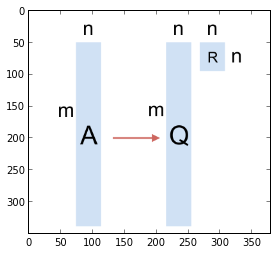
\includegraphics[width=0.7\textwidth]{stat_AtA_qr_files/stat_AtA_qr_fig_01.png}
\par
\end{center}
\end{codeoutput}
\end{codecell}
Q hesabi icin biraz daha takla atmak lazim,
\[A = QR\]\[AR^{-1} = QRR^{-1} \]\[Q = AR^{-1} \]
Demek ki $R$'i elde ettikten sonra onu tersine cevirip (inverse) $A$ ile
carparsak, bu bize $Q$'yu verecek. Dert degil, $R$ ufak bir matris,
$n \times n$, ve tersini alma operasyonu pahali bir islem olsa da bu
boyutlarda yavas olmaz. Daha sonra bu $R^{-1}$'i alip bu sefer baska bir
esle/indirge ile carpim islemine tabi tutariz. R'yi direk alttaki script
icine yazdik (B olarak) bir sonuc ortaminda bu verinin baska bir sekilde
MRJob islemine verilmis olmasi lazim. Bir isleme zinciri var, zincirde
once $A^TA$, Cholesky, oradan $R$ alinip baska bir isleme (job)
aktariliyor.

\begin{codecell}
\begin{codeinput}
\begin{lstlisting}
print (open("AB.py").read())
\end{lstlisting}
\end{codeinput}
\begin{codeoutput}
\begin{verbatim}
from mrjob.job import MRJob
from mrjob.protocol import PickleProtocol
import numpy as np, sys

class MRAB(MRJob):
    INTERNAL_PROTOCOL = PickleProtocol
    
    def __init__(self, *args, **kwargs):
        super(MRAB, self).__init__(*args, **kwargs)
        self.buffer_size = 4
        self.n = 4
        self.data = []
        # an example B
        self.B = np.array([[-20.49390153,   0.        ,   0.        ,   0.        ],
                           [-22.59208669,  -5.25334361,   0.        ,   0.        ],
                           [-12.88188096, -11.41585875,   4.44244436,   0.        ],
                           [-12.93067597, -12.53849977,   2.54158031,  -4.37310096]])

        
    def mapper(self, key, line):
        line_vals = map(np.float,line.split())
        self.data.append(line_vals)
        if len(self.data) == self.buffer_size:
            mult = np.dot(self.data,self.B.T)
            self.data = []
            yield (key, mult)
    
    def reducer(self, key, tokens):
        for x in tokens:
            yield (key, str(x))
    
if __name__ == '__main__':
    MRAB.run()
\end{verbatim}
\end{codeoutput}
\end{codecell}
\begin{codecell}
\begin{codeinput}
\begin{lstlisting}
!python AB.py A_matrix
\end{lstlisting}
\end{codeinput}
\begin{codeoutput}
\begin{verbatim}
using configs in /home/burak/.mrjob.conf
creating tmp directory /tmp/AB.burak.20130926.111826.388978
writing to /tmp/AB.burak.20130926.111826.388978/step-0-mapper_part-00000
\end{verbatim}
\begin{verbatim}
Counters from step 1:
  (no counters found)
writing to /tmp/AB.burak.20130926.111826.388978/step-0-mapper-sorted
> sort /tmp/AB.burak.20130926.111826.388978/step-0-mapper_part-00000
writing to /tmp/AB.burak.20130926.111826.388978/step-0-reducer_part-00000
Counters from step 1:
  (no counters found)
Moving /tmp/AB.burak.20130926.111826.388978/step-0-reducer_part-00000 -> /tmp/AB.burak.20130926.111826.388978/output/part-00000
Streaming final output from /tmp/AB.burak.20130926.111826.388978/output
null	"[[ -61.48170459  -88.78963451  -62.09685608  -84.98432736]\n [ -20.49390153  -27.8454303   -19.85529535  -27.30069639]\n [ -40.98780306  -55.6908606   -39.7105907   -54.60139278]\n [-184.44511377 -250.6088727  -205.35232431 -234.71714361]]"
null	"[[ -61.48170459  -99.29632173  -76.04368486 -131.21677204]\n [ -40.98780306  -55.6908606   -39.7105907   -54.60139278]\n [-184.44511377 -250.6088727  -205.35232431 -234.71714361]\n [ -61.48170459  -88.78963451  -62.09685608 -102.4767312 ]]"
null	"[[-184.44511377 -250.6088727  -205.35232431 -234.71714361]\n [ -61.48170459  -99.29632173  -76.04368486 -131.21677204]\n [ -40.98780306  -55.6908606   -39.7105907   -54.60139278]\n [-184.44511377 -250.6088727  -205.35232431 -234.71714361]]"
null	"[[ -61.48170459  -88.78963451  -62.09685608 -102.4767312 ]\n [ -61.48170459  -88.78963451  -62.09685608  -84.98432736]\n [ -61.48170459  -99.29632173  -76.04368486 -131.21677204]\n [ -40.98780306  -55.6908606   -39.7105907   -54.60139278]]"
removing tmp directory /tmp/AB.burak.20130926.111826.388978
\end{verbatim}
\end{codeoutput}
\end{codecell}
Kontrol edelim,

\begin{codecell}
\begin{codeinput}
\begin{lstlisting}
B = np.array([[-20.49390153,   0.        ,   0.        ,   0.        ],
              [-22.59208669,  -5.25334361,   0.        ,   0.        ],
              [-12.88188096, -11.41585875,   4.44244436,   0.        ],
              [-12.93067597, -12.53849977,   2.54158031,  -4.37310096]])
np.dot(A,B.T)
\end{lstlisting}
\end{codeinput}
\begin{codeoutput}
\begin{verbatim}
array([[ -61.48170459,  -88.78963451,  -62.09685608, -102.4767312 ],
       [ -61.48170459,  -88.78963451,  -62.09685608,  -84.98432736],
       [ -61.48170459,  -99.29632173,  -76.04368486, -131.21677204],
       [ -40.98780306,  -55.6908606 ,  -39.7105907 ,  -54.60139278],
       [-184.44511377, -250.6088727 , -205.35232431, -234.71714361],
       [ -61.48170459,  -99.29632173,  -76.04368486, -131.21677204],
       [ -40.98780306,  -55.6908606 ,  -39.7105907 ,  -54.60139278],
       [-184.44511377, -250.6088727 , -205.35232431, -234.71714361],
       [ -61.48170459,  -99.29632173,  -76.04368486, -131.21677204],
       [ -40.98780306,  -55.6908606 ,  -39.7105907 ,  -54.60139278],
       [-184.44511377, -250.6088727 , -205.35232431, -234.71714361],
       [ -61.48170459,  -88.78963451,  -62.09685608, -102.4767312 ],
       [ -61.48170459,  -88.78963451,  -62.09685608,  -84.98432736],
       [ -20.49390153,  -27.8454303 ,  -19.85529535,  -27.30069639],
       [ -40.98780306,  -55.6908606 ,  -39.7105907 ,  -54.60139278],
       [-184.44511377, -250.6088727 , -205.35232431, -234.71714361],
       [ -81.97560612, -116.63506481,  -90.83704015, -126.11438629]])
\end{verbatim}
\end{codeoutput}
\end{codecell}
Carpimlar ayni. Yanliz dikkat, satirlarin sirasi degisik olabilir,
burada problem esle/indirge isleminin $A$'yi parcalama sonucu her carpim
parcasinin degisik bir sirada ele geciyor olmasi. Eger siralamayi ayni
$A$ gibi istiyorsak, bu sira no'sunu $A$ verisi icinde ilk satira koymak
lazim ve esleyiciler oradan alip bu no'yu anahtar olarak yayinlamalilar.
Bu eklemeyi okuyucuya birakiyorum!

Simdi QR hesabini bu sekilde yapip yapamayacagimizi kontrol edelim. Eger
qr ile $Q$ hesaplarsak,

\begin{codecell}
\begin{codeinput}
\begin{lstlisting}
q,r = lin.qr(A)
q
\end{lstlisting}
\end{codeinput}
\begin{codeoutput}
\begin{verbatim}
array([[-0.14638501, -0.13188879,  0.36211188, -0.35057934],
       [-0.14638501, -0.13188879,  0.36211188,  0.56410341],
       [-0.14638501, -0.51259871, -0.16600517, -0.02328772],
       [-0.09759001,  0.03897744,  0.26737941, -0.1251395 ],
       [-0.43915503,  0.1753985 , -0.14740047,  0.02394349],
       [-0.14638501, -0.51259871, -0.16600517, -0.02328772],
       [-0.09759001,  0.03897744,  0.26737941, -0.1251395 ],
       [-0.43915503,  0.1753985 , -0.14740047,  0.02394349],
       [-0.14638501, -0.51259871, -0.16600517, -0.02328772],
       [-0.09759001,  0.03897744,  0.26737941, -0.1251395 ],
       [-0.43915503,  0.1753985 , -0.14740047,  0.02394349],
       [-0.14638501, -0.13188879,  0.36211188, -0.35057934],
       [-0.14638501, -0.13188879,  0.36211188,  0.56410341],
       [-0.048795  ,  0.01948872,  0.1336897 , -0.06256975],
       [-0.09759001,  0.03897744,  0.26737941, -0.1251395 ],
       [-0.43915503,  0.1753985 , -0.14740047,  0.02394349],
       [-0.19518001, -0.11240007,  0.04559899, -0.21745867]])
\end{verbatim}
\end{codeoutput}
\end{codecell}
$R$'in tersi ile $A$ carpilinca hakikaten $Q$ elde ediliyor mu? Kontrol
edelim.

\begin{codecell}
\begin{codeinput}
\begin{lstlisting}
np.dot(A,lin.inv(B.T))
\end{lstlisting}
\end{codeinput}
\begin{codeoutput}
\begin{verbatim}
array([[-0.14638501, -0.13188879,  0.36211188, -0.35057934],
       [-0.14638501, -0.13188879,  0.36211188,  0.56410341],
       [-0.14638501, -0.51259871, -0.16600517, -0.02328772],
       [-0.09759001,  0.03897744,  0.26737941, -0.1251395 ],
       [-0.43915503,  0.1753985 , -0.14740047,  0.02394349],
       [-0.14638501, -0.51259871, -0.16600517, -0.02328772],
       [-0.09759001,  0.03897744,  0.26737941, -0.1251395 ],
       [-0.43915503,  0.1753985 , -0.14740047,  0.02394349],
       [-0.14638501, -0.51259871, -0.16600517, -0.02328772],
       [-0.09759001,  0.03897744,  0.26737941, -0.1251395 ],
       [-0.43915503,  0.1753985 , -0.14740047,  0.02394349],
       [-0.14638501, -0.13188879,  0.36211188, -0.35057934],
       [-0.14638501, -0.13188879,  0.36211188,  0.56410341],
       [-0.048795  ,  0.01948872,  0.1336897 , -0.06256975],
       [-0.09759001,  0.03897744,  0.26737941, -0.1251395 ],
       [-0.43915503,  0.1753985 , -0.14740047,  0.02394349],
       [-0.19518001, -0.11240007,  0.04559899, -0.21745867]])
\end{verbatim}
\end{codeoutput}
\end{codecell}
Sonuclar birebir ayni.

Ustteki teknikleri kullanarak artik devasa boyutlarda satiri olan bir
$A$ matrisi uzerinde artik QR hesabi yapabilirsiniz.

\subsection{SVD}

Peki $QR$ sonuclarini kullanarak SVD sonuclarini alabilir miyiz? SVD
bize ne verir?
\[ A = U \Sigma V^T \]
$U$ ve $V^T$ ortogonal matrislerdir, $\Sigma$ sadece kosegeni boyunca
degerleri olan bir matristir. Daha fazla detay icin Lineer Cebir Ders
29'a bakabilirsiniz. Simdi $A = QR$ yerine koyalim,
\[ QR =  U \Sigma V^T \]\[ R = Q^T U \Sigma V^T \]
Bu son formuled $Q^TU$ formulu, iki ortogonal matrisin carpimidir.
Lineer Cebir kurallarina gore iki ortogonal matrisin carpimi bir diger
ortogonal matristir. Bu yeni ortogonal matrise $U_R$ adi verelim, o
zaman
\[ R = U_R \Sigma V^T \]
Bu son formul bize bir seyler soyluyor. $R$'nin SVD uzerinden
ayristirilabilecegini soyluyor ve bu ayristirma sonrasi ele gecen
$U_R,V^T$ ve $\Sigma$ kosegen matrisleridir! Bu cok onemli bir sonuc. Bu
ayristirmanin sonucu $A$'nin ki ile birbirine cok benziyor, tek fark $U$
ile $U_1$. Bu iki matris arasindaki gecis soyle:
\[ U_R = Q^T U \]\[ U = QU_R \]
\begin{codecell}
\begin{codeinput}
\begin{lstlisting}
imshow(imread('ur.png'))
\end{lstlisting}
\end{codeinput}
\begin{codeoutput}
\begin{verbatim}
<matplotlib.image.AxesImage at 0x2dc64d0>
\end{verbatim}
\begin{center}
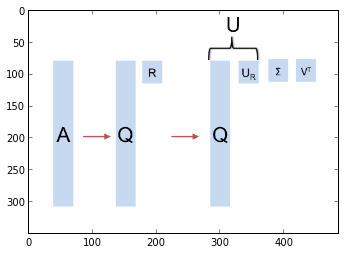
\includegraphics[width=0.7\textwidth]{stat_AtA_qr_files/stat_AtA_qr_fig_02.png}
\par
\end{center}
\end{codeoutput}
\end{codecell}
Bu demektir ki eger $R$ uzerinde kutuphanemizin svd cagrisini
kullanirsak (ki $R$ nispeten ufak oldugu icin bu ucuz olur) ele gecen
$U_R$'i alip, $Q$ ile carparsak, $A$ ayristirmasinin $U$'sunu elde
ederiz! $Q$ ile carpim esle/indirge uzerinden yapilabilir, fakat basit
bir carpim islemi oldugu icin paralelize edilmesi kolaydir (ustteki
mrjob script'inde yaptigimiz gibi).

\subsubsection{Yansitmak}

Peki son olarak, eger $m \times n$ durumunda $n$ bile cok buyukse ne
yapacagiz? Bu durumda $A$ matrisini daha ufak bir boyuta ``yansitmak
(project)'' bir cozum olabilir. Eger bu daha az olan boyut ``yeterince
yuksek'' ise (ki burada ``yeterince'' ifadesi verinin icerigine
baglidir), o zaman veri noktalari arasindaki mesafelerin pek degismedigi
matematiksel olarak ispatlanmistir {[}3{]}. Eger elimizde 10 milyar
satir, 1 milyar kolon var ise, $k = 100$ secebiliriz, ve bundan sonra
ustte gosterilen Cholesky ve SVD cagrilari $n \times n$,
$100 \times 100$ uzerinden yapilacaktir, ve bu herhangi bir bilgisayarin
idare edebilecegi bir boyuttur. Rasgele matris olusturmak ve yansitma
yapma ornegi altta.

\begin{codecell}
\begin{codeinput}
\begin{lstlisting}
import numpy.random as rand

n = 4; k = 2

Omega = rand.randn(n,k)

A = np.loadtxt('A_matrix')

Y = np.dot(A, Omega)

print "Y", Y.shape

\end{lstlisting}
\end{codeinput}
\begin{codeoutput}
\begin{verbatim}
Y (17, 2)
\end{verbatim}
\end{codeoutput}
\end{codecell}
Kaynaklar

{[}1{]} Benson, A., Tall-and-skinny Matrix Computations in MapReduce

{[}2{]} Constantine, P. G., Gleich, D. F. , Tall and Skinny QR
factorizations in MapReduce architectures

{[}3{]} Dasgupta, S., Gupta, A., An Elementary Proof of a Theorem of
Johnson and Lindenstrauss

\end{document}
